\documentclass[oneside]{book}

\usepackage{amssymb}
\usepackage{graphicx}

\begin{document}
\title{Notes and Solutions for ``Measure Theory and Integration" by Michael E. Taylor}
\author{Arya Pourzanjani} 
\date{\today}
\maketitle

%%%%%%%%%%%%%%%%
%%%%%%%%%%%%%%%%
\chapter{The Riemann Integral}
%%%%%%%%%%%%%%%%
%%%%%%%%%%%%%%%%

\section*{Solutions}
\begin{enumerate}
%%%%%%%%%
%%%%%%%%%
\item[7.] Since $f:[ac,bc]\to \mathbb{R}$ is Riemann integrable, by definition its integral is equal to its upper sum i.e.

\begin{eqnarray}
\label{eq:upperSumStretched}
\frac{1}{c}\int_{ac}^{bc} f(x)\,dx &=& \frac{1}{c} \inf_{\cal{P}} \bar{I}_{\cal{P}}(f) \nonumber \\
&=& \frac{1}{c} \inf_{\cal{P}} \sum_{k} \sup_{[x_k,x_{k+1}]} f(x)\, l([x_k,x_{k+1}])
\end{eqnarray}

Assume $c > 1$ for the sake of intuition here. They key insight to note here is that by multiplying the input of a function by a constant i.e. $f(cx)$ we effectively make it so that when going from left to right the function ``reaches" the numbers in its range earlier than it normally would and the function appears shrunken. Figure \ref{fig:sinSpedUp} shows an example.

\begin{figure}[h]
    \centering
    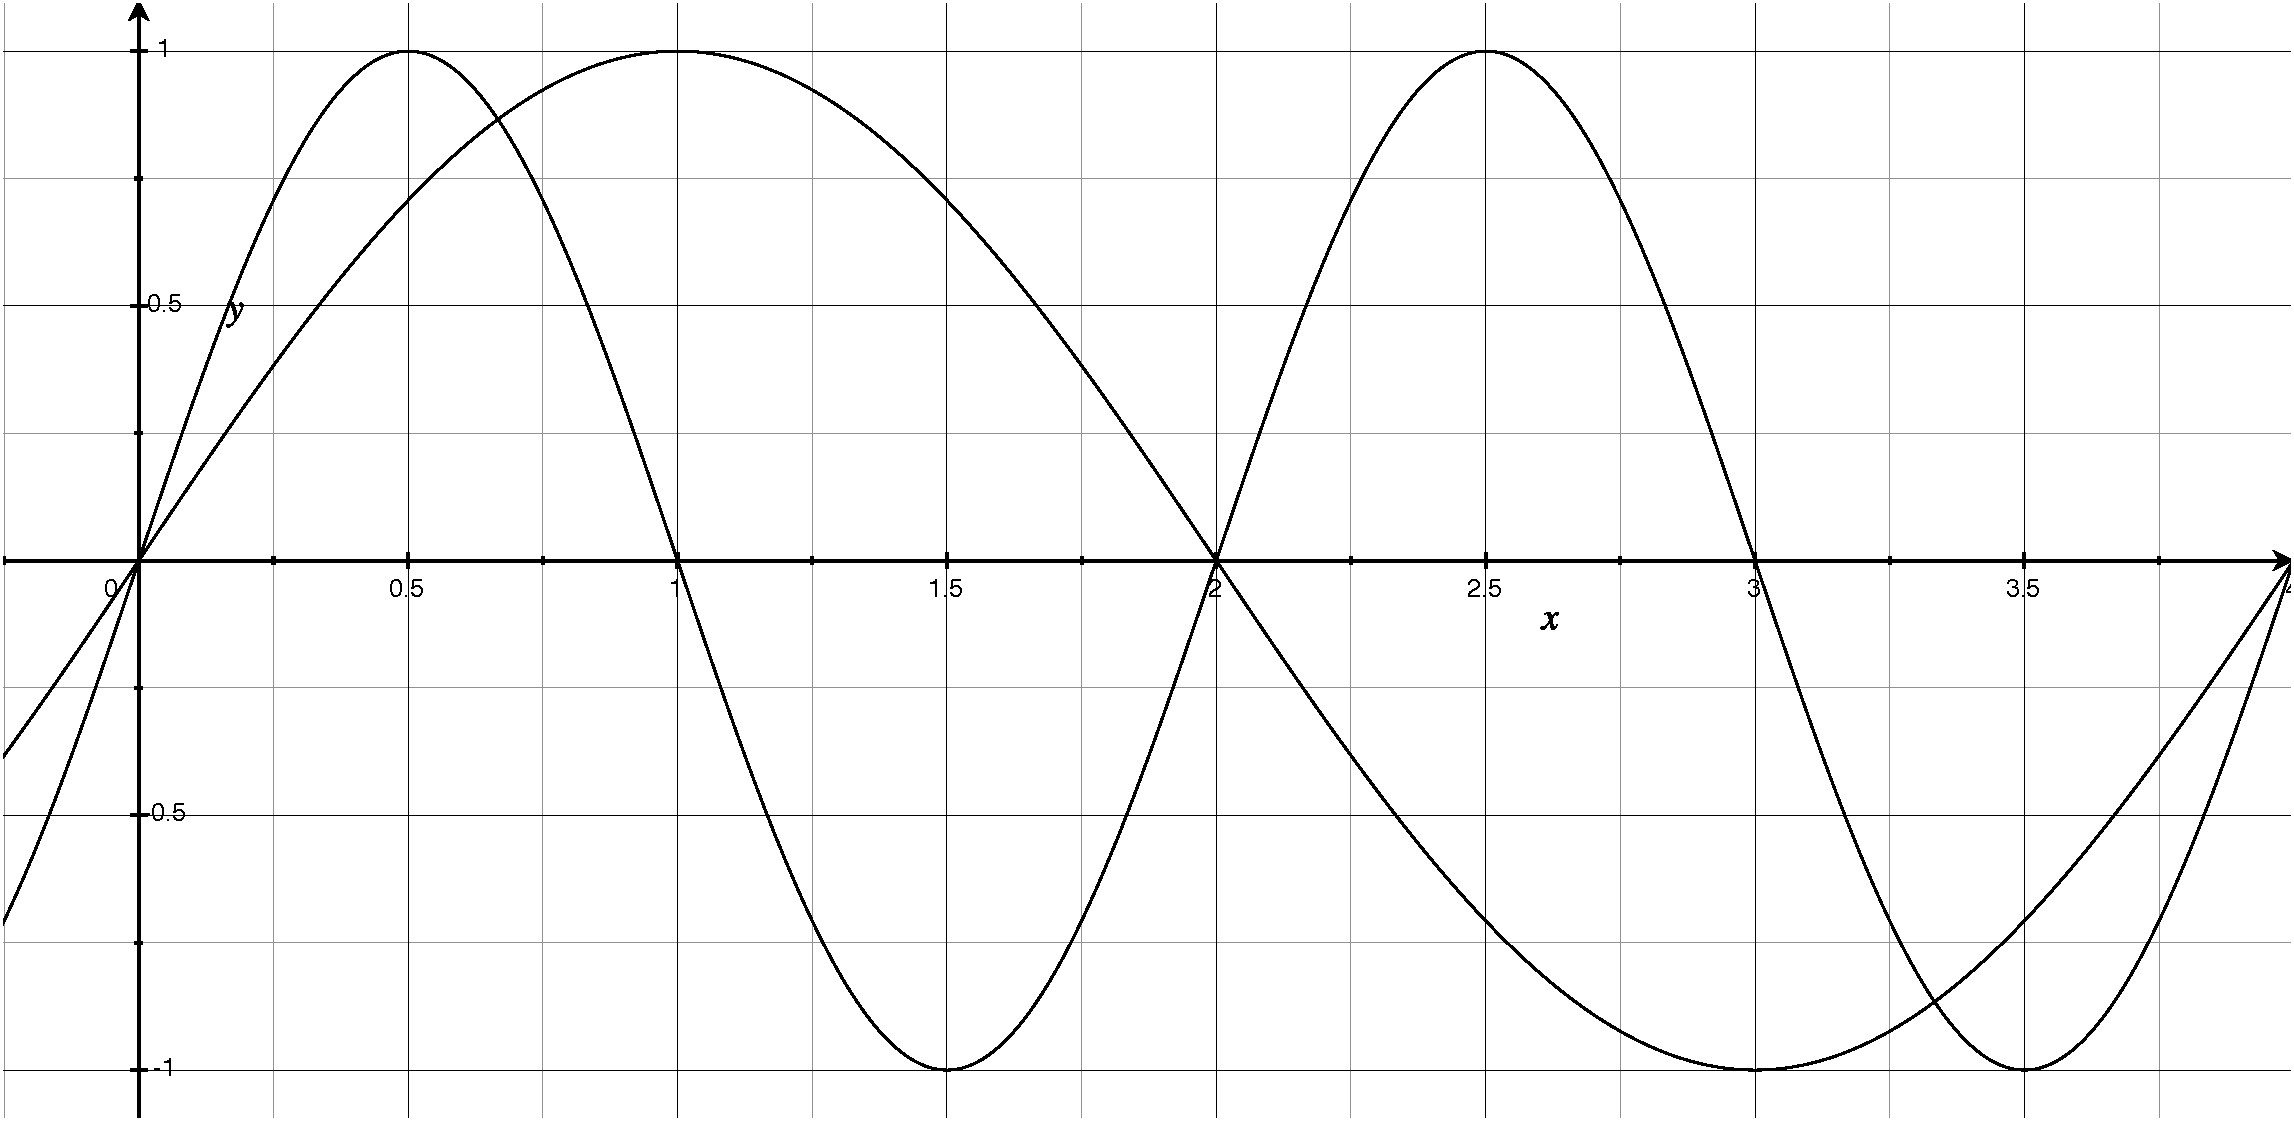
\includegraphics[width=0.6\textwidth]{sinSpeedUp.pdf}
    \caption{Graph of $\sin(\pi x/2)$ and it's ``sped up" or ``shrunken" counterpart $\sin(\pi x/2)$}
    \label{fig:sinSpedUp}
\end{figure}

Since $f(cx)$ reaches elements in its range earlier (and ``faster") than its stretched counterpart $f(x)$, the range of $f(x)$ over an interval $[x_k,x_{k+1}]$ is equivalent to the range of $f(cx)$ over the earlier and smaller interval $\left[\frac{x_k}{c},\frac{x_{k+1}}{c}\right]$. So equation \ref{eq:upperSumStretched} is equivalent to

\begin{eqnarray}
\label{eq:upperSumShrunk}
&& \frac{1}{c} \inf_{\cal{P}} \sum_{k} \sup_{\left[\frac{x_k}{c},\frac{x_{k+1}}{c}\right]} f(cx)\, l([x_k,x_{k+1}]) \nonumber \\
&=& \inf_{\cal{P}} \sum_{k} \sup_{\left[\frac{x_k}{c},\frac{x_{k+1}}{c}\right]} f(cx)\, l\left(\left[\frac{x_k}{c},\frac{x_{k+1}}{c}\right]\right)
\end{eqnarray}

The last equality comes from the fact that the length of $[x_k,x_{k+1}]$ is equal to the length of its shrunken counterpart multiplied by the shrink factor $c$. The shrink factor then cancelled out with the $1/c$ at the front of the expression.

Now it is clear though that equation \ref{eq:upperSumShrunk} is by definition $\bar{I}(f(cx))$. A parallel argument can be made for the lower sum and thus the equality is shown. Adding another term $d$ to the input make the function reach points in its range earlier, thus the function will be shifted to the left.

%%%%%%%%%
%%%%%%%%%
\item[8.] $f$ is continuous, which just means that if the two points \\$(x_1,s_1),(x_2,s_2) \in I \times S$ are less than a certain distance apart i.e. $d_{I \times S}((x_1,s_1),(x_2,s_2)) < \delta$ then $| f(x_1,s_1)-f(x_2,s_2) | < \omega(\delta)$. Now we need to show that $\varphi(y)$ has this same property, that is we need to show that if $d_S(s_1,s_2) < \delta$ then

\begin{eqnarray}
\label{eq:phiContinuous}
\left| \varphi(s_1) - \varphi(s_2) \right| &=& \left| \int_I f(x,s_1)\, dx - \int_I f(x,s_2)\, dx \right | < \omega(\delta)
\end{eqnarray}

Now we note that $d_{I \times S}((x,s_1),(x,s_2))=d_S(s_1,s_2)$ so if $d_S(s_1,s_2) < \delta$ then $d_{I \times S}((x,s_1),(x,s_2))< \delta$. Then from the continuity of $f$ this implies that $|f(x,s_1)-f(x,s_2)| < \omega(\delta)$, which in turn implies that

\begin{eqnarray}
&&\left| \int_I f(x,s_1)-f(x,s_2)\, dx \right | < l(I)\omega(\delta) \nonumber \\
&\Rightarrow& \left| \int_I f(x,s_1)\,dx- \int_I f(x,s_2)\, dx \right | < l(I)\omega(\delta) \nonumber \\
&\Rightarrow& \left| \varphi(s_1) - \varphi(s_2) \right| < l(I)\omega(\delta)
\end{eqnarray}

but this is exactly the property of continuity (equation \ref{eq:phiContinuous}) we wanted to show (up to a constant $l(I)$). The constant here is irrelevant because in words continuity means that the function can be as close as desired by making the inputs sufficiently close. The constant being there just means that we'd have to make the inputs a little closer to ensure the outputs are as close as we need them to be, but none the less we can ensure the outputs will be as arbitrarily close as need be.

%%%%%%%%%
%%%%%%%%%
\item[9.] Again we need to show that if  $d_S(s_1,s_2) < \delta$ then

\begin{eqnarray}
\label{eq:phi2Continuous}
&&\left| \varphi(s_1) - \varphi(s_2) \right| \nonumber\\
&=&\left| \int_{g_0(s_1)}^{g_1(s_1)} f(x,s_1)\, dx - \int_{g_0(s_2)}^{g_1(s_2)} f(x,s_2)\, dx \right |
\end{eqnarray}

Since $a \le g_0(y) < g_1(y) \le b$ these integrals are can be thought of as being evaluated over an interval that is to the right of $a$ by $\alpha_j := g_0(s_j)-a$ and smaller than $[a,b]$ by a factor of $\kappa_j :=l([g_0(s_j),g_1(s_j)])/l([a,b])$. From exercise 7 we know that we can stretch these functions and divide by the stretching factor to get an equivalent size interval. We can also translate the function the right to the left and still have an equivalent integral. By doing the latter first we see that \ref{eq:phi2Continuous} is equivalent to

\begin{eqnarray}
\left| \int_{a}^{g_1(s_1)-\alpha_1} f(x+\alpha_1,s_1)\, dx - \int_{a}^{g_1(s_2)-\alpha_2} f(x+\alpha_2,s_2)\, dx \right |
\end{eqnarray}

which by stretching is equivalent to

\begin{eqnarray}
\left| \frac{1}{\kappa_1} \int_{a}^{b} f\left(\frac{x+\alpha_1}{\kappa_1},s_1\right)\, dx - \frac{1}{\kappa_2} \int_{a}^{b} f\left(\frac{x+\alpha_2}{\kappa_2},s_2\right)\, dx \right|
\end{eqnarray}

and this is just the familiar condition \ref{eq:phiContinuous} from exercise 8 with a couple constant scalars that will not affect the limit.

%%%%%%%%%
%%%%%%%%%
\item[10.]

\end{enumerate}
%%%%%%%%%%%%%%%%
%%%%%%%%%%%%%%%%
\chapter{Lebesgue Measure on the Line}
%%%%%%%%%%%%%%%%
%%%%%%%%%%%%%%%%

\end{document}